\chapter{Landasan Teori}

\section{FHIR (Fast Healthcare Interoperability Resources)}
FHIR \textit{(Fast Healthcare Interoperability Resources)} menurut \cite{mark_l_braunstein_fhir_2022} adalah standar pertukaran data kesehatan yang dikembangkan oleh HL7 (Health Level Seven International). FHIR dapat digunakan untuk mengintegrasikan sistem kesehatan yang berbeda dan mengijinkan pertukaran data yang cepat dan aman antara sistem yang berbeda.
\begin{figure}[H]
    \centering
    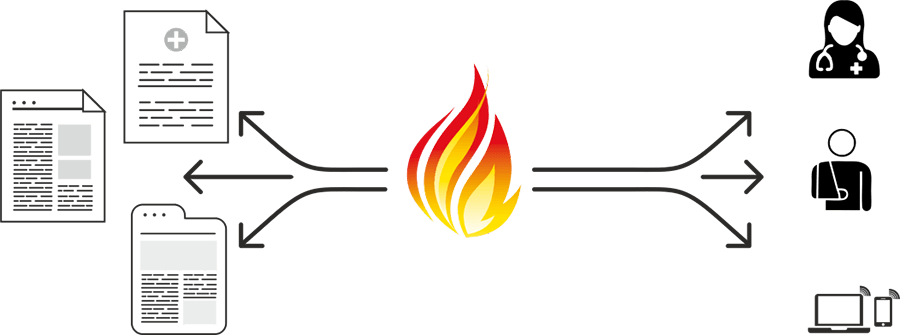
\includegraphics[width=0.8\textwidth]{contents/chapter-3/FHIR-img-1.png}
    \caption{Gambaran FHIR}
    \label{fig:fhir}
\end{figure}
FHIR menyediakan kumpulan resource yang dapat digunakan untuk pertukaran data kesehatan, seperti informasi pasien, informasi medis, dan informasi billing. Resource ini dapat ditransmisikan dalam format yang berbeda, seperti JSON atau XML. FHIR juga menyediakan API (Application Programming Interface) yang dapat digunakan untuk mengakses data dan layanan yang tersedia melalui jaringan.

FHIR dapat digunakan untuk meningkatkan interoperabilitas sistem kesehatan dan mengijinkan data kesehatan untuk ditransmisikan dengan cepat dan aman antara sistem yang berbeda. Standar ini juga memudahkan pengembangan aplikasi yang dapat mengakses data kesehatan dari berbagai sumber dan digunakan dalam berbagai konteks, seperti telemedicine, pengelolaan kesehatan, dan analisis data kesehatan.


\section{Machine-to-Machine (M2M) Authentication}
Machine-to-Machine (M2M) authentication adalah proses verifikasi yang digunakan untuk mengautentikasi perangkat atau mesin yang terhubung ke jaringan, seperti komputer, perangkat IoT, atau perangkat mobile. Proses ini memastikan bahwa hanya perangkat yang sah yang dapat terhubung ke jaringan dan mengakses data atau layanan yang tersedia seperti skema pada Gambar \ref*{fig:m2m}.

M2M authentication dapat menggunakan berbagai metode, seperti pengenalan suara, pengenalan wajah, pengenalan sidik jari, atau kombinasi dari metode tersebut. Dalam beberapa kasus, M2M authentication juga dapat menggunakan teknologi kriptografi, seperti enkripsi atau sertifikat digital, untuk memastikan keamanan komunikasi antar perangkat.
\begin{figure}
    \centering
    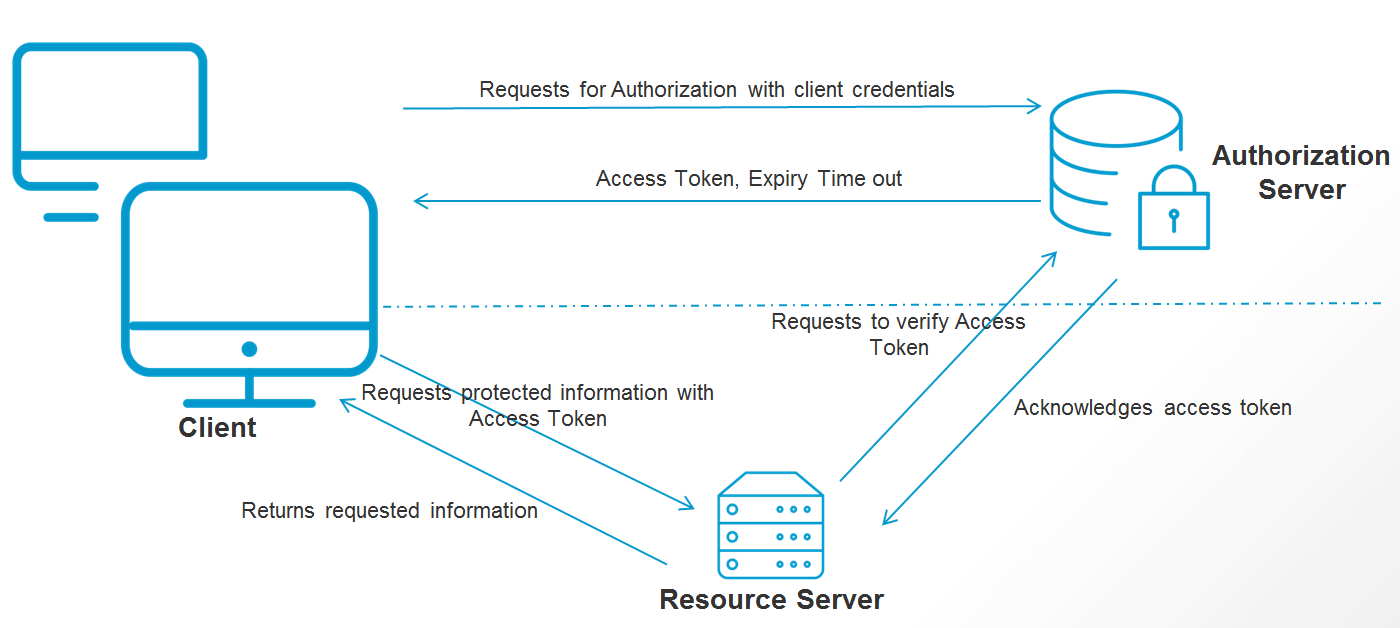
\includegraphics[width=0.8\textwidth]{contents/chapter-3/m2m_auth.png}
    \caption{Skema M2M Authentication}
    \label{fig:m2m}
\end{figure}

M2M authentication juga dapat digabungkan dengan metode risk-based authentication untuk meningkatkan keamanan sistem. Dengan menganalisis faktor- faktor yang dapat meningkatkan risiko, seperti lokasi geografis, waktu akses, dan jenis perangkat yang digunakan, sistem dapat mengambil tindakan yang sesuai untuk menangani ancaman potensial.

\section{Klien Kredensial}
Klien membuat permintaan ke server otorisasi dengan mengirimkan ID klien, rahasia klien, bersama dengan audiens dan klaim-klaim lainnya. Server otorisasi memvalidasi permintaan tersebut, dan, jika berhasil, mengirimkan respons dengan token akses. Klien sekarang dapat menggunakan token akses untuk meminta sumber daya yang dilindungi dari server sumber daya.
Karena klien harus selalu menjaga rahasia klien, pemberian ini hanya dimaksudkan untuk digunakan pada klien terpercaya. Dengan kata lain, klien yang menyimpan rahasia klien harus selalu digunakan di tempat di mana tidak ada risiko rahasia tersebut disalahgunakan. Sebagai contoh, meskipun mungkin ide yang baik untuk menggunakan hibah kredensial klien di sistem internal yang mengirimkan laporan di seluruh web ke bagian lain dari sistem Anda, namun tidak dapat digunakan untuk alat publik yang dapat diakses oleh pengguna eksternal mana pun.
Berikut ini adalah permintaan HTTP yang relevan pada Tabel \ref{tab:req_http} berikut:

\begin{table}[H]
    \caption{Permintaan HTTP}
    \vspace{0.5em}
    \centering
    \begin{tabular}{|c|c|c|}
        \hline
        Permintaan & Deskripsi \\
        \hline \hline
        POST & Metode HTTP \\
        \hline
        /token & Endpoint \\
        \hline
        grant\_type=client\_credentials & Jenis hibah \\
        \hline
        & ID klien \\
        \hline
        & Rahasia klien \\
        \hline
        & Audiens \\
        \hline
    \end{tabular}
    \label{tab:req_http}
\end{table}

Sedangkan berikut contoh respon HTTP yang relevan pada Tabel \ref{tab:res_http} berikut:

\begin{table}[h]
    \caption{Respon HTTP}
    \vspace{0.5em}
    \centering
    \begin{tabular}{|c|c|c|}
        \hline
        Respon & Deskripsi \\
        \hline \hline
        200 OK & Kode status HTTP \\
        \hline
        Content-Type: application/json & Header HTTP \\
        \hline
        Cache-Control: no-store & Header HTTP \\
        \hline
        Pragma: no-cache & Header HTTP \\
        \hline
        \{ & Body \\
        \hline
        "access\_token": "2YotnFZFE & \\
        \hline
        "token\_type": "example", & \\
        \hline
        "expires\_in": 3600, & \\
        \hline
        "example\_parameter": "example\_value" & \\
        \hline
        \} & \\
        \hline
    \end{tabular}
    \label{tab:res_http}
\end{table}

\section{\textit{Risk Based Authentication}}
Risk-based adalah suatu metode yang digunakan untuk mengukur dan
mengelola risiko. Dalam konteks keamanan, risk-based authentication adalah metode autentikasi yang mengukur tingkat risiko dari suatu permintaan akses, dan mengambil tindakan yang sesuai berdasarkan tingkat risiko tersebut. Metode ini bertujuan untuk mengenali dan menangani ancaman potensial tanpa mengekang fleksibilitas dan kenyamanan pengguna.
Dalam konteks Machine-to-Machine (M2M) authentication, risk-based authentication digunakan untuk mengukur tingkat risiko dari suatu permintaan akses dan mengambil tindakan yang sesuai berdasarkan tingkat risiko tersebut.
Prosesnya dapat dilakukan dengan cara menganalisis faktor-faktor yang dapat meningkatkan risiko, seperti lokasi geografis, waktu akses, dan jenis perangkat yang digunakan.
Setelah tingkat risiko diukur, sistem dapat mengambil tindakan yang sesuai. Jika tingkat risiko dianggap rendah, maka autentikasi dapat dilakukan secara otomatis tanpa intervensi manusia. Namun, jika tingkat risiko dianggap tinggi, maka autentikasi dapat dilakukan dengan cara yang lebih ketat, seperti mengharuskan verifikasi melalui kode SMS atau panggilan telepon, atau pembatasan akses sesuai dengan level risiko.
Risk-based authentication juga dapat digabungkan dengan metode analisis risiko dinamis, yaitu mengukur risiko secara real-time dan mengambil tindakan sesuai dengan situasi yang ada. Ini dapat membantu sistem untuk mengenali dan menangani ancaman potensial secara efektif tanpa mengekang fleksibilitas dan kenyamanan pengguna seperti ilustrasi pada Gambar 3.2.

Bagian ini membahas pertimbangan etis penelitian dan [potensi] masalah serta
keterbatasannya. Jika menyangkut penelitian dengan makhluk hidup, maka dibutuhkan adanya \textit{ethical clearance}, di bagian ini hal itu akan dibahas. Demikian juga tentang keterbatasan ataupun masalah yang akan timbul.

\section{\textit{Classification and Regression Tree (CART)}}
Metode CART merupakan suatu metode pohon keputusan (decision tree) yang bersifat recursive partitioning. Satu tree terdiri atas tiga komponen utama yaitu root node, internal node dan terminal node. Pada metode CART simpul akar (root node) dipartisi menjadi dua simpul anak (internal node), masing-masing simpul anak kemudian dipartisi menjadi dua simpul anak yang baru hingga menjadi terminal node yang bersifat homogen sebagai interpretasi dari tree Zhang, H \& Singer (2010). CART membentuk tree dengan dua langkah yaitu, pembentukan maksimal dari decision tree berdasarkan proses splitting (pemilahan) dan pemangkasan (pruning) dengan mempertimbangkan tree dan cabang pohon yang terbentuk. Proses splitting variabel pada percabangan node pada tree dilihat dari variabel yang memiliki nilai goodness of split maksimal. Nilai ini dilihat berdasarkan perubahan gini impurity/gini index pada node t dan percabangan nodenya menurut Gordon dkk. (1984) dengan rumus sebagai berikut.
%insert equation
\\
Node Kiri:
\begin{equation}
    \text{imp}(\mathbf{t}_{\text{L}}) = \sum_{l=1}^{2} p_{\text{tL}}(l)(1 - p_{\text{tL}}(l))
\end{equation}
\\
Node Kanan:
\begin{equation}
    \text{imp}(\mathbf{t}_{\text{R}}) = \sum_{l=1}^{2} p_{\text{tR}}(l)(1 - p_{\text{tR}}(l))
    \end{equation}
\\ 
Node t:
\begin{equation}
    \text{imp}(\mathbf{t}) = \sum_{k=1}^{2} p_{\text{t}}(k)(1 - p_{\text{t}}(k))
    \end{equation}
\\
Keterangan:
\begin{equation}
    p_{t}(k) = \frac{n_{t}(k)}{n_{t}} \quad \text{dan} \quad p_{t}(l) = \frac{n_{t}(l)}{n_{t}}
    \end{equation}
\\
\begin{equation}
    p_{t}(k), p_{t}(l) : \text{Proporsi objek kelas klasifikasi ke-} k \text{ atau ke-} l \text{ pada node } t
    \end{equation}
    
    \begin{equation}
    n_{t}(k), n_{t}(l) : \text{Jumlah observasi kelas klasifikasi ke-} k \text{ atau ke-} l \text{ pada node } t
    \end{equation}
    
    \begin{equation}
    n_{t} : \text{Jumlah seluruh observasi pada node } t
    \end{equation}
    

Gini Impurity berfungsi untuk menentukan seberapa banyak pemisah yang akan dibentuk decision tree. Sementara dalam pemilihan variabel s yang digunakan untuk memilah ditentukan oleh nilai Goodness of Split sebagai berikut.
%insert equation
\begin{equation}
    \Delta\text{imp}(\mathbf{s}, \mathbf{t}) = \text{imp}(\mathbf{t}) - \text{p}_{t\text{L}}\text{imp}(\mathbf{t}_{\text{L}}) - \text{p}_{t\text{R}}\text{imp}(\mathbf{t}_{\text{R}})
    \end{equation}
Keterangan:
\begin{equation}
    p_{t\text{L}} = \frac{n_{t\text{L}}}{n_{t}} \quad \text{and} \quad p_{t\text{R}} = \frac{n_{t\text{R}}}{n_{t}}
    \end{equation}
\\
\begin{equation}
    p_{t}(\text{L atau R}) : \text{Proporsi objek pada node } t \text{ yang memilah pada node } t_{\text{L}} \text{ atau node } t_{\text{R}}
    \end{equation}
    
    \begin{equation}
    n_{t}(\text{L atau R}) : \text{Jumlah observasi pada node } t \text{ yang memilah pada node } t_{\text{L}} \text{ atau node } t_{\text{R}}
    \end{equation}
    
    \begin{equation}
    n_{t} : \text{Jumlah seluruh observasi pada node } t
    \end{equation}
    
Variabel pemilah s yang memiliki goodness of split maksimal merupakan variabel yang lebih baik digunakan untuk melakukan proses splitting. Serta apabila terminal node yang terbentuk dari internal node memiliki nilai gini index lebih besar maka sebaiknya proses splitting dihentikan pada internal node sehingga menjadi terminal node.

\subsection{Random Forest}
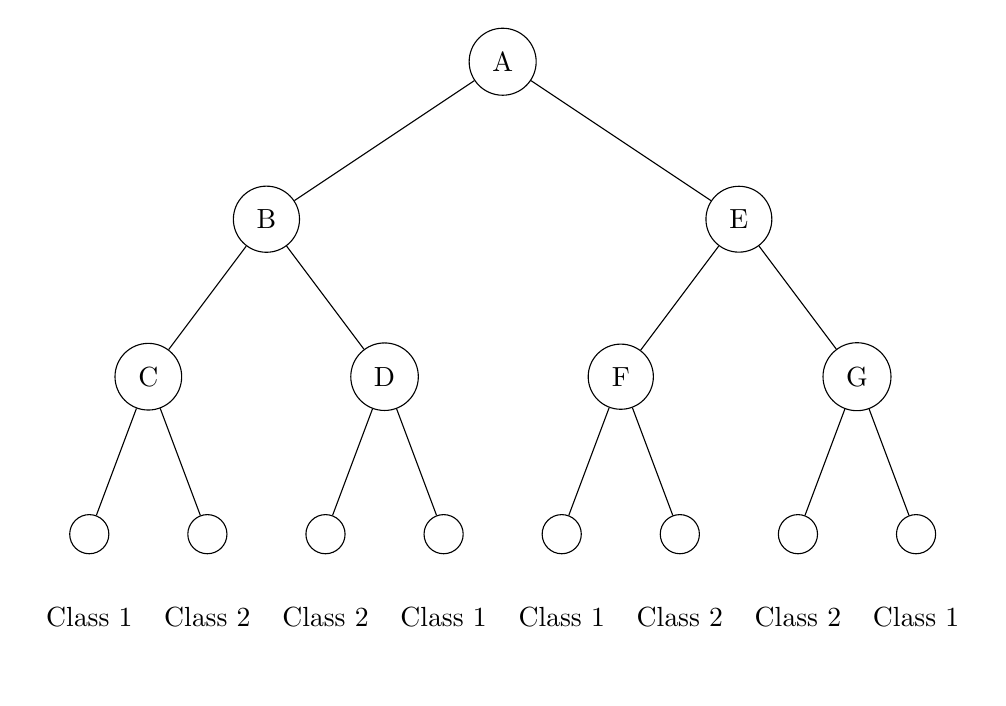
\begin{tikzpicture}[
    grow=down,
    level 1/.style={sibling distance=6cm, level distance=2cm},
    level 2/.style={sibling distance=3cm, level distance=2cm},
    level 3/.style={sibling distance=1.5cm, level distance=2cm},
    every node/.style={draw, circle, inner sep=0.5em}
  ]
  
  % Root node
  \node {A}
    child {
      node {B}
      child {
        node {C}
        child {node[label=below:Class 1] {}}
        child {node[label=below:Class 2] {}}
      }
      child {
        node {D}
        child {node[label=below:Class 2] {}}
        child {node[label=below:Class 1] {}}
      }
    }
    child {
      node {E}
      child {
        node {F}
        child {node[label=below:Class 1] {}}
        child {node[label=below:Class 2] {}}
      }
      child {
        node {G}
        child {node[label=below:Class 2] {}}
        child {node[label=below:Class 1] {}}
      }
    };
  
  \end{tikzpicture}

Membentuk tree lainnya sehingga terbentuk beberapa tree berdasarkan ntree Random Forest (RF) merupakan pengembangan metode CART. RF merupakan kumpulan banyak decision tree untuk membangun satu forest dan melihat vote klasifikasi dari tree yang menghasilkan prediktif lebih akurat Genuer dkk. (2008). Tree di RF dibentuk tidak menggunakan seluruh sampel melainkan menggunakan sampel bootstrap dan tidak melakukan pruning. Bootstrap merupakan metode berbasis resampling data dengan syarat pengembalian dalam menyelesaikan suatu permasalahan James dkk. (2021). Pada RF sampel bootstrap yang digunakan adalah 2/3 data original dengan pengembalian sehingga membentuk sampel bootstrap yang memiliki jumlah sama dengan data original sedangkan 1/3 data original lainnya disebut sampel out of bag (OOB) yang digunakan untuk pengujian prediksi tree yang sudah terbentuk dari sampel bootstrap Breiman (2001).
Terdapat tiga tuning parameter yang digunakan metode RF yaitu mtry (banyak input variabel secara acak terpilih dalam satu node pemilahan) yang secara default mtry = $\sqrt{p}$ untuk kasus klasifikasi, ntree (jumlah banyaknya tree dalam forest) yang secara default ntree = 500, penelitian ini menggunakan ntree berjumlah 100, 250, 500, dan 1000, serta node size (minimum nomor observasi dalam sebuah node) yang secara default 1 untuk klasifikasi Probst dkk. (2019). Pembentukan tree pada RF dilakukan dengan cara membentuk sampel bootstrap, lalu melakukan teknik recursive partitioning pada sampel bootstrap sehingga menghasilkan sebuah tree, dimana dalam proses splitting tree atribut diambil berdasarkan banyaknya variabel yang terpilih melalui mtry. Selanjutnya, melakukan kembali pembentukan sampel bootstrap dan metode recursive partitioning untuk dalam membangun satu forest untuk melihat vote klasifikasi dari seluruh tree yang terbentuk.

\subsection{Laju Galat Klasifikasi}
OOB sampel berfungsi sebagai percobaan prediksi tree yang terbentuk dikarenakan setiap tree memiliki sampel bootstrap yang berbeda, sehingga setiap amatan dapat menjadi sampel OOB dan perlu diprediksi menggunakan beberapa tree yang dibangun tidak menggunakan sampel tersebut. Estimasi error pada hasil prediksi RF dapat diduga dengan menggunakan laju galat OOB (OOB error rate) yang dihitung dari hasil proporsi kesalahan prediksi klasifikasi setiap amatan dari hasil RF Janitza \& Hornung (2018). Penggunaan mtry untuk melihat hasil dari OOB error diharapkan tidak terlalu rendah, dikarenakan apabila terlalu rendah, maka hasil OOB error akan semakin tinggi yang menghasilkan RF memiliki kinerja yang buruk. OOB error rate diharapkan memiliki nilai terkecil (minimum). Berikut perhitungan laju galat OOB dalam klasifikasi.

\begin{equation}
    \text{Laju Galat } \text{OOB}_i = \frac{1}{n} \sum_{i=1}^{n} \mathbb{I}(Y_i \neq P_i)
    \end{equation}

OOB error rate digunakan untuk memprediksi observasi ke- $i$ dari $Xi$ dimana
prediksi hanya berlaku untuk suatu tree yang sampel bootstrapnya tidak mengandung ($Xi$, $Yi$)
    
\subsection{\textit{Variable Importance Measure (VIM)}}
Penggunaan analisis dalam RF secara umum sangat sulit untuk melakukan interpretasi dalam memperoleh informasi. Salah satu solusi untuk mempermudah memperoleh informasi dalam RF ialah dengan mengidentifikasi Variable Importance Measure (VIM) untuk variabel prediktor. Apabila variabel importance dapat diidentifikasi, maka hasil RF akan diperoleh metode penyeleksian variabel yang berpengaruh penting terhadap pembentukan tree dalam RF. Estimasi pemilihan variabel importance dalam random forest dapat dilakukan dengan melihat berapa banyak kenaikan prediksi error (OOB) data untuk variabel terpilih sementara yang lainnya tidak berubah Liaw \& Wiener (2002).
Metode representatif dari perhitungan pengukuran variabel importance adalah Mean Decrease Impurity (MDI) atau disebut juga dengan Mean Decrease Gini (MDG) yang diusulkan oleh Breiman pada tahun 2001. Suatu p peubah penjelas dengan h=(1,2,…,p) maka rumus mengukur tingkat kepentingan peubah penjelas Xh dengan cara berikut (Xiao Li. dkk, 2019).